\newcommand{\fgLabelledCycle}[1]{
\begin{tikzpicture}
\def \n {#1}
\def \r {2cm}
\def \sp {14}
\def \tt {360/\n}

\foreach \s in {0,...,\numexpr#1-1\relax}
{
\node[draw, circle] at ({\tt * \s}:\r) {$[\s]$};
\draw[->, >=latex] ({\tt * \s + \sp}:\r)
arc ({\tt * \s + \sp}:{\tt * (\s + 1) - \sp}:\r);
}
\end{tikzpicture}}

\newcommand{\fgClock}{
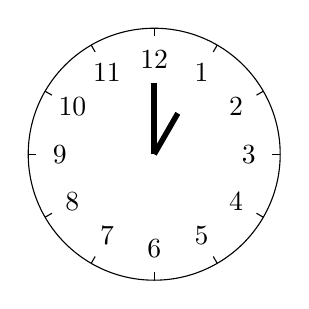
\begin{tikzpicture}
% draw clock border
\draw (0,0) circle [radius=1.6cm];

% draw clock label
\foreach \angle [count=\i] in {60,30,...,-270}
{
\draw (\angle:1.5cm) -- (\angle:1.6cm);
\node at (\angle:1.2cm) {\i};
}

% draw hands
\draw[line width=2pt] (60:0) -- (60:0.6cm);
\draw[line width=2pt] (90:0) -- (90:0.9cm);
\end{tikzpicture}}

\newcommand{\fgNumberLine}[2]{
\begin{tikzpicture}
\foreach \x in {#1,...,#2}
{
\draw (\x, -0.1) -- (\x, 0.1);
\node at (\x, -0.4) {$\x$};
}
\draw (#1, 0) -- (#2, 0);

% bold line at zero
\draw[line width=2pt] (0, -0.15) -- (0, 0.15);
\end{tikzpicture}}

\newcommand{\fgLineSegment}{
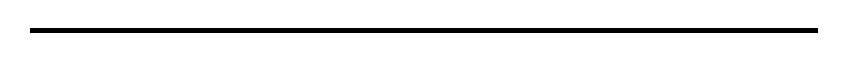
\begin{tikzpicture}
\draw[line width=2pt] (-5, 0) -- (5, 0);
\end{tikzpicture}}

\newcommand{\fgLine}{
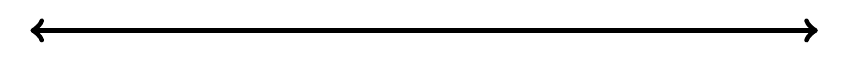
\begin{tikzpicture}
\draw[->, =>latex, line width=2pt] (0, 0) -- (5, 0);
\draw[->, =>latex, line width=2pt] (0, 0) -- (-5, 0);
\end{tikzpicture}}

\newcommand{\fgRay}{
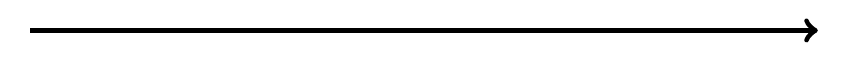
\begin{tikzpicture}
\draw[->, =>latex, line width=2pt] (-5, 0) -- (5, 0);
\end{tikzpicture}}

\newcommand{\fgTwoRays}{
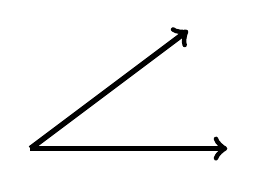
\begin{tikzpicture}
\draw[->, =>latex, line width=2pt] (0, 0) -- (2.5, 0);
\draw[->, =>latex, line width=2pt] (0, 0) -- (2, 1.5);
\end{tikzpicture}}

\newcommand{\fgTwoRaysFar}{
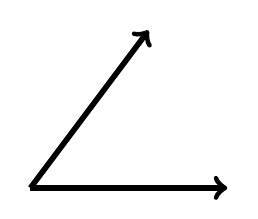
\begin{tikzpicture}
\draw[->, =>latex, line width=2pt] (0, 0) -- (2.5, 0);
\draw[->, =>latex, line width=2pt] (0, 0) -- (1.5, 2);
\end{tikzpicture}}

\newcommand{\fgTwoRaysRight}{
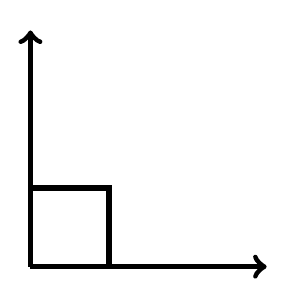
\begin{tikzpicture}
\draw[->, =>latex, line width=2pt] (0, 0) -- (3, 0);
\draw[->, =>latex, line width=2pt] (0, 0) -- (0, 3);
\draw[line width=2pt] (0, 1) -- (1, 1) -- (1, 0);
\end{tikzpicture}}

\newcommand{\fgAsterisk}{
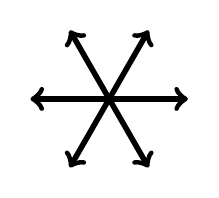
\begin{tikzpicture}
\draw[->, =>latex, line width=2pt] (0, 0) -- (1, 0);
\draw[->, =>latex, line width=2pt] (0, 0) -- (0.5, 0.87);
\draw[->, =>latex, line width=2pt] (0, 0) -- (-0.5, 0.87);
\draw[->, =>latex, line width=2pt] (0, 0) -- (-1, 0);
\draw[->, =>latex, line width=2pt] (0, 0) -- (-0.5, -0.87);
\draw[->, =>latex, line width=2pt] (0, 0) -- (0.5, -0.87);
\end{tikzpicture}}

\newcommand{\fgAngleN}[1]{
\begin{tikzpicture}
\coordinate (A) at (0,0);
\coordinate (B) at (0:3);
\coordinate (C) at (#1:3);
\draw[->, =>latex, line width=2pt] (A) -- (B);
\draw[->, =>latex, line width=2pt] (A) -- (C);
\pic [draw, line width=2pt, "{\small\SI{#1}{\degree}}", angle radius=1.5cm] {angle = B--A--C};
\end{tikzpicture}}

\newcommand{\fgAngleSumNM}[2]{
\begin{tikzpicture}
\coordinate (A) at (0,0);
\coordinate (B) at (0:3);
\coordinate (C) at (#1:3);
\coordinate (D) at (#1+#2:3);
\draw[->, =>latex, line width=2pt] (A) -- (B);
\draw[->, =>latex, line width=2pt] (A) -- (C);
\draw[->, =>latex, line width=2pt] (A) -- (D);
\pic [draw, line width=2pt, "{\small\SI{#1}{\degree}}", angle radius=1.5cm] {angle = B--A--C};
\pic [draw, line width=2pt, "{\small\SI{#2}{\degree}}", angle radius=1.5cm] {angle = C--A--D};
\pic [draw=blue, line width=1pt, angle radius=2.0cm] {angle = B--A--D};
\end{tikzpicture}}

\newcommand{\fgAngleDiffNM}[2]{
\begin{tikzpicture}
\coordinate (A) at (0,0);
\coordinate (B) at (0:4);
\coordinate (C) at (#1:4);
\coordinate (D) at (#1-#2:4);
\draw[->, =>latex, line width=2pt] (A) -- (B);
\draw[->, =>latex, line width=2pt] (A) -- (C);
\draw[->, =>latex, line width=2pt] (A) -- (D);
\pic [draw, line width=2pt, "{\small\SI{#1}{\degree}}", angle radius=2.3cm] {angle = B--A--C};
\pic [draw, line width=2pt, "{\small\SI{#2}{\degree}}", angle radius=1.0cm] {angle = D--A--C};
\pic [draw=blue, line width=1pt, angle radius=2.0cm] {angle = B--A--D};
\end{tikzpicture}}

\newcommand{\fgTriangle}[3]{
\begin{tikzpicture}
  \coordinate (A) at #1;
  \coordinate (B) at #2;
  \coordinate (C) at #3;
  \draw[line width=.5mm] (A) -- (B) -- (C) -- cycle;
\end{tikzpicture}}

\newcommand{\fgRightTriangleWithLegs}[5]{
\begin{tikzpicture}
  \coordinate (A) at #1;
  \coordinate (B) at #2;
  \coordinate (C) at #3;
  \draw[line width=.5mm] (A) -- node[below] {#4} (B) -- node[right] {#5} (C) --
  cycle;
  \tkzMarkRightAngle[draw=red](A,B,C)
\end{tikzpicture}}

\newcommand{\fgTriangleAlt}[3]{
\begin{tikzpicture}
  \coordinate (A) at #1;
  \coordinate (B) at #2;
  \coordinate (C) at #3;
  \coordinate (HA) at ($(B)!(A)!(C)$);
  \coordinate (HB) at ($(A)!(B)!(C)$);
  \coordinate (HC) at ($(B)!(C)!(A)$);
  \draw[line width=.5mm] (A) -- (B) -- (C) -- cycle;
  \draw[red,line width=.3mm]
    (A) -- (HA)
    (B) -- (HB)
    (C) -- (HC);
  \tkzMarkRightAngle[draw=red](B,HC,C)
  \tkzMarkRightAngle[draw=red](C,HA,A)
  \tkzMarkRightAngle[draw=red](A,HB,B)
\end{tikzpicture}}

\newcommand{\fgBoxedTriangle}[5]{
\begin{tikzpicture}
  \coordinate (A) at #1;
  \coordinate (B) at #2;
  \coordinate (C) at #3;
  \coordinate (D) at #4;
  \coordinate (E) at #5;
  \coordinate (HA) at ($(B)!(A)!(C)$);
  \coordinate (HB) at ($(A)!(B)!(C)$);
  \coordinate (HC) at ($(B)!(C)!(A)$);
  \draw[fill=orange!30] (A) rectangle (C);
  \draw[fill=purple!30] (A) rectangle (B);
  \draw[line width=.5mm,fill=white,fill opacity=0.4]
    (A) -- (B) -- (C) -- cycle;
  \draw[blue,line width=.3mm] (B) -- (C) -- (D) -- (E) -- cycle;
  \draw[red,line width=.3mm] (A) -- (HA);
  \tkzMarkRightAngle[draw=red](C,HA,A)
\end{tikzpicture}}

\newcommand{\fgQuadrilateral}[4]{
\begin{tikzpicture}
  \coordinate (A) at #1;
  \coordinate (B) at #2;
  \coordinate (C) at #3;
  \coordinate (D) at #4;
  \draw[line width=.5mm] (A) -- (B) -- (C) -- (D) -- (A) -- (B);
\end{tikzpicture}}

\newcommand{\fgQuadrilateralDiag}[4]{
\begin{tikzpicture}
  \coordinate (A) at #1;
  \coordinate (B) at #2;
  \coordinate (C) at #3;
  \coordinate (D) at #4;
  \draw[line width=.5mm] (A) -- (B) -- (C) -- (D) -- (A) -- (B);
  \draw[line width=.5mm] (C) -- (A);
\end{tikzpicture}}
